\section{Auswertung}
\label{sec:auswertung}
In diesem Teil werden die Messwerte der verschiedenen Schlatungen vorgestellt und erläutert.
Dabei wird in der Reihenfolge der Durchführung vorgegangen.
\subsection{Fehlerrechung}

\subsection{invertierter Linearverstärker}
Als erste Schaltung wird der invertierter Linearverstärker aufgebaut.
Der Aufbau wird in Abschnitt \section{sec:durchfuehrung} im Detail erklärt.
Für die Schaltung werden drei Messungen durchgeführt.
Dabei werden die Widerstände ausgetauscht um unterschiedliche Spannungsverstärkungen zu erzielen.

Die genutzten Widerstände der verschiedenen Messungen sind in Tabelle \ref{tab:wider_inv_lin} zu sehen.
\begin{table}
    \centering
    \begin{tabular}{ccc}
        \toprule
        Messung & $R_1 \, / \, k\Omega $ & $R_2 \, / \,  k\Omega $ \\
        \midrule 
        1 & 1 & 100 \\
        2 & 47 & 100 \\
        3 & 47 & 220 \\
        \bottomrule
    \end{tabular}
    \caption{Die genutzen Widerstände für den invertierter Linearverstärker für drei Messdurchgänge.}
    \label{tab:wider_inv_lin}
\end{table}
Bei den Messdurchgänge werden, wie in Abschnitt \ref{sec:durchfuehrung} beschrieben, für verschiedenen Frequenzen die Phase zwischen Eingangsspannung $U_\text{in}$ und Ausgangsspannung $U_\text{out}$, sowie die Höhe der Ausgangsspannung gemessen.
Danach wird aus dem Quotienten der Eingangsspannung und Ausgangsspannung die Verstärkung $V'$ nach Gleichung \ref{eq:ampli} berechnet.
Die Verstärkung ist in Form eines doppelt logarithmischen Plots in Abbildung \ref{fig:inv_lin} zu sehen.
\begin{figure}
    \centering
    \begin{subfigure}{0.49\linewidth}%
        \includegraphics[width=\textwidth]{build/inv_lin_1.pdf}
        \subcaption{Messwerte der Messung 1.}
    \end{subfigure}
    \hfill
    \begin{subfigure}{0.49\linewidth}%
        \includegraphics[width=\textwidth]{build/inv_lin_2.pdf}
        \subcaption{Messwerte der Messung 2.}
    \end{subfigure}\\
    \begin{subfigure}{0.49\linewidth}%
        \includegraphics[width=\textwidth]{build/inv_lin_3.pdf}
        \subcaption{Messwerte der Messung 3.}
    \end{subfigure}
    \caption{Die Messwerte der Verstärkung durch den invertierten Linearverstärkers. Es wird die Verstärkung gegen die Frequenz der Eingangsspannung geplottet.
    Dies geschieht in einer Plot mit doppelt logarithmischer Achse. Ein Fit wird für den abfallenden Bereich angefertigt, welcher als blaue Linie zu erkennen ist.}
    \label{fig:inv_lin}
\end{figure}
Die Ausgleichfunktion für die Messwerte wird mithilfe der Funktion
\begin{equation}
    Fit(f) = a f^b
    \label{eq:fit}
\end{equation}
durchgeführt, wobei $f$ die Frequenz ist.
Die Ausgleichrechung ergibt für die Parameter $a$ und $b$ der verschiedenen Messreiehen die Widerstände
\begin{align}
    Fit_1(f) &= \SI{6.9(28)e5}{\frac{\V}{\Hz}} f^{-\SI{1.02(4)}{}} \\
    Fit_2(f) &= \SI{5.7e8}{\frac{\V}{\Hz}} f^{-1.51}\\
    Fit_3(f) &= \SI{1.2e4}{\frac{\V}{\Hz}} f^{-0.68}
\end{align}
Aufgrund der doppelt logarithmischen Achsen und der geringen Anzahl von Messwerten im abfallenden Bereich, könne für Messung 2 und 3 durch die Funktion 'curve\_fit' des python Pakets 'scipy' \cite{scipy} keine Unsicherheiten bestimmt werden.
Für den Plateubereich, welcher für geringe Frequenzen im invertierten Linearverstärker erkennbar ist wird der Mittelwert der Verstärkung berechnet.
Bei der Berechnung der Mittelwerte werden dabei unterschiedlich viele Messwerte genutzt, je nachdem wie lang das Plateu bei der jeweiligen Konfiguration ist.
In Tabelle \ref{tab:inv_lin_mittel} sind die berechneten Mittelwerte aufgetragen. 
In der Tabelle sind zudem die Anzahl der genutzten Messpunkte der jeweiligen Messung, sowie die theoretische Verstärkung zu sehen.
Die theoretische Verstärkung wird dabei nach Gleichung \eqref{eq:verstaerkung} berechnet.
Zudem wird die Grenzfrequenz 
\begin{equation*}
  f_\text{Grenz} = \sqrt(V_\text{theo}')/a)**(1/b)
\end{equation*}
berechnet, wobei $V_\text{theo}'$ die nach Gleichung \eqref{eq:verstaerkung} berechnete Verstärkung für die gegebene Schaltung ist.
In der Tabelle ist außerdem das Bandbreitenprodukt
\begin{equation*}
    B = f_\text{Grenz}\bar{V}'
\end{equation*}
aufgezeigt.
\begin{table}
    \centering
    \begin{tabular}{cccccc}
        \toprule
        Messung & Anzahl Messpunkte & Mittelwert $\bar{V}'$ & theoretische Verstärkung $V_\text{theo}'$ & Grenzfrequenz $f_\text{Grenz}$ & Bandbreitenprodukt $B$\\
        \midrule
        1 & 4 & $\SI{93.600(2100)}{}$ & 100 & $\SI{79763.77(5000)}{\Hz}$ & $\SI{74.77(5000)e5}{\Hz}$\\
        2 & 8 & $\SI{2.080(0)}{} $& 2.126 & $\SI{166918.65}{\Hz} $& $\SI{3.47e5}{\Hz}$\\
        3 & 7 & $\SI{4.680(50)}{} $& 4.680 &$\SI{50399.22}{\Hz}$ & $\SI{2.35(24)e5}{}$\\
        \bottomrule 
    \end{tabular}
    \label{tab:inv_lin_mittel}
\end{table} 
Abgesehen von der Ausgangsspannung, aus der die Verstärkung berechnet wird, wird auch die Phase zwischen Eingangsspannung und Ausgangsspannung gemessen.
Diese wird anschließend gegen die logarithmische  Frequenz aufgetragen.
Die resultierenden Plots sind in Abbildung \ref{fig:phase} zu sehen.
\begin{figure}
    \centering
    \begin{subfigure}{0.49\linewidth}%
        \includegraphics[width=\textwidth]{build/inv_lin_phase1.pdf}
        \subcaption{Messwerte der Messung 1.}
    \end{subfigure}
    \hfill
    \begin{subfigure}{0.49\linewidth}%
        \includegraphics[width=\textwidth]{build/inv_lin_phase2.pdf}
        \subcaption{Messwerte der Messung 2.}
    \end{subfigure}\\
    \begin{subfigure}{0.49\linewidth}%
        \includegraphics[width=\textwidth]{build/inv_lin_phase3.pdf}
        \subcaption{Messwerte der Messung 3.}
    \end{subfigure}
    \caption{Die Messwerte der Phase zwischen Eingangsspannung und Ausgangsspannung beim invertierten Linearverstärkers. Die Phase wird gegen die Frequenz der Eingangsspannung geplottet.
    Dies geschieht in einer Plot mit logarithmischer y-Achse.}
    \label{fig:phase}
\end{figure}
In den Plots ist zu erkennen, dass es für kleine Frequenz ein Plateu für Phase $\approx 180\,\si{\degree}$ gibt.
Bei höheren Frequenzen fällt die Phase exponentiell ab, bis diesem einen geringen Wert von $(0-40)\,\si{\degree}$ erreicht hat.

\subsection{Umkehr Integrator}
Die nächste Schaltung die untersucht wird ist der Umkehr Integrator.
Für diesen wird der Aufbau gemäß \ref{sec:durchfuehrung} umgebaut.
Daraufhin wird die Frequenz der Eingangsspannung varriert und die Ausgangsspannung gemessen.
Diese wird in Abbildung \ref{fig:inv_int} gegen die Frequenz in einem doppelt logarithmischen Plot aufgetragen.
Durch die Werte wird ein Fit gelegt welcher für die Funktion \eqref{eq:fit} angefertigt wird.
Die Fit Parameter ergeben die Funktion
\begin{align*}
    Fit_4(f) = \SI{54.4(15)}{\frac{\V}{\Hz}} f^{\SI{-0.737(15)}{}} \, .
\end{align*}

\begin{figure}
    \centering
    \includegraphics[width=\textwidth]{build/inv_int.pdf}
    \caption{Die gemessene Ausgangsspannung $U_\text{out}$ des Umkehr Integrators wird in einem doppelt logarithmischen Plot gegen die Frequenz aufgetragen.
    Ein Fit wird durch den linear Abfallenden Bereich des doppelt logarithmischen Plots gelegt, welcher als blaue Gerade zu sehen ist.}
    \label{fig:inv_int}
\end{figure}

Um zu erkennen ob der Umkehr Integrator die Stammfunktion des Eingangssignals bildet, werden eine Sinus-, Dreiecks- und eine Rechteckspannung an den Umkehr Integrator angelegt.
Die Ausgangsspannung wird mit einem Oszilloskop gemessen.
Die Bilder, welches das Oszilloskop produziert, können in Abbildung \ref{fig:umkehr_oszi} eingesehen werden.
\begin{figure}
    \centering
    \begin{subfigure}{0.49\linewidth}%
        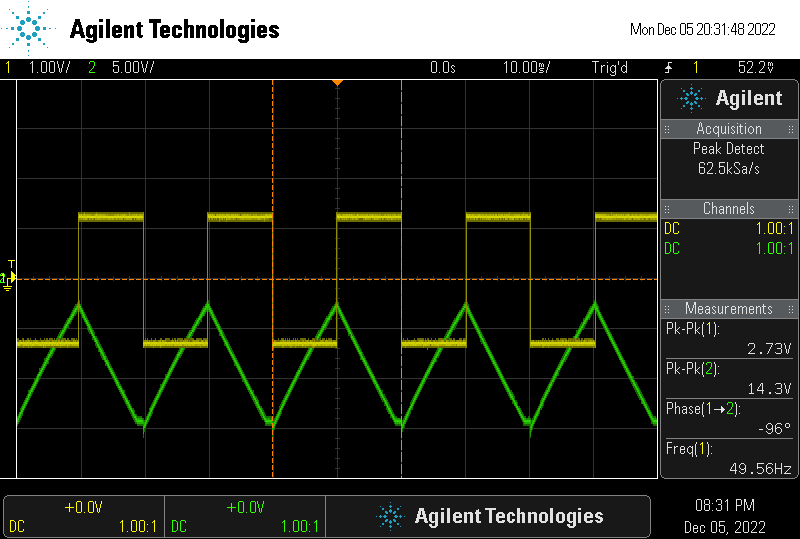
\includegraphics[width=\textwidth]{data/Int_rechteck.png}
        \subcaption{Das Eingangssignals ist eine Rechteckspannung, das Ausgangssignal eine Dreiecksspannung.}
    \end{subfigure}
    \hfill
    \begin{subfigure}{0.49\linewidth}%
        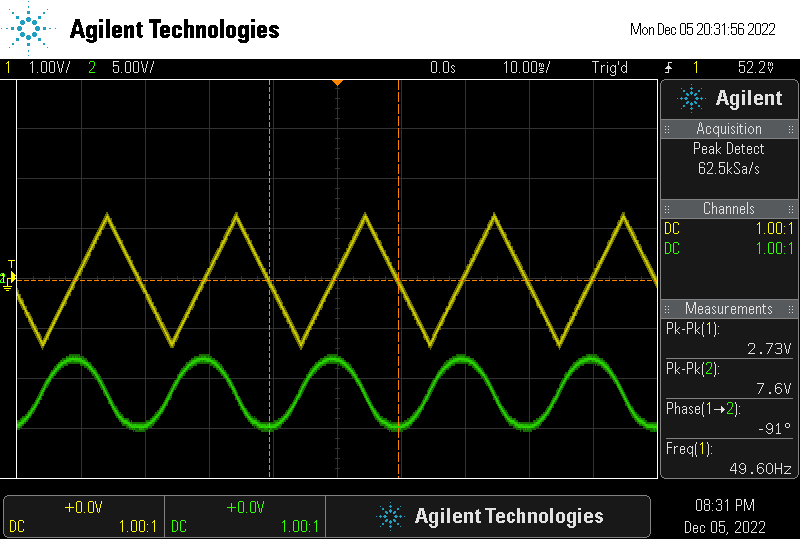
\includegraphics[width=\textwidth]{data/int_dreieck.png}
        \subcaption{Das Eingangssignals ist eine Dreiecksspannung, das Ausgangssignal ist eine Rechteckspannung.}
    \end{subfigure}\\
    \begin{subfigure}{0.49\linewidth}%
        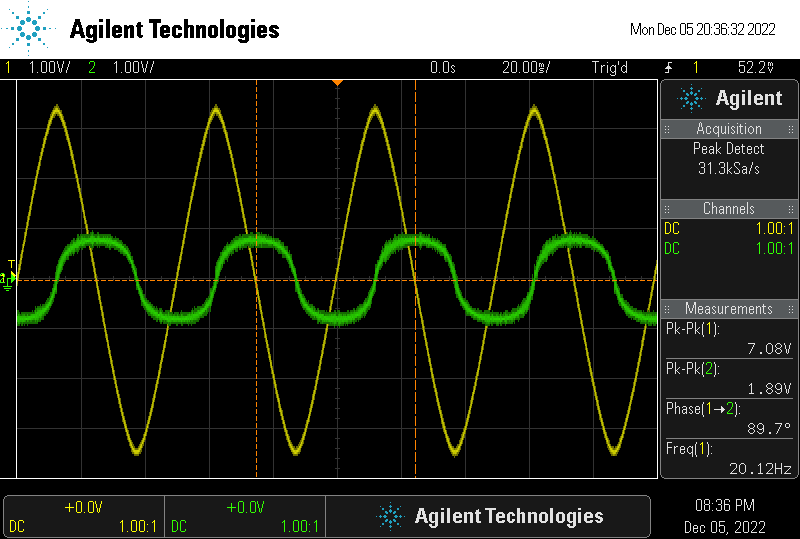
\includegraphics[width=\textwidth]{data/int_sinus.png}
        \subcaption{Das Eingangssignal ist eine Sinusspannung, das Ausgangssignal ist ein Cosinussignal.}
    \end{subfigure}
    \caption{Die Bildschirmfotos des Oszilloskop bei verschiedenen Eingangssignals und Ausgangssignalen.
    Das gelbe Signal ist dabei immer das Eingangssignals des Umkehr Integrators, das grüne Signal ist das Ausgangssignal der Schaltung.}
    \label{fig:umkehr_oszi}
\end{figure}
Die erwartete Eigenschaft des bilden der Stammfunktion des Eingangssignals ist zu erkennen.

\subsection{invertierender-Differenzierer}
Nun wird die Schaltung eines invertierenden-Differenzieres, wie in \ref{sec:durchfuehrung} beschrieben, aufgebaut.
Bei dem Messvorgang wird genauso wie zuvor beim Umkehr Integrator vorgegangen.
Die gemessene Ausgangsspannung wird wieder gegen die Frequenz in einem doppelt logarithmischen Plots aufgetragen, welcher in Abbildung \ref{fig:inv_dif} zu sehen ist.
\begin{figure}
    \centering
    \includegraphics[width=\textwidth]{build/inv_diff.pdf}
    \caption{Die Ausgangsspannung des invertierenden-Differenzieres wird doppelt logarithmisch gegen die Frequenz aufgetragen.
    Ein Fit wird durch die Messwerte gelegt welcher als blaue Gerade zu sehen ist.}
    \label{fig:inv_diff}
\end{figure}
Es wird ein Fit nach Funktion \eqref{eq:fit} angefertigt, dieser ergibt sich zu 
\begin{equation*}
    Fit_5 = \SI{0.0058(22)}{\frac{\V}{\Hz}} f^{\SI{1.09(5)}{}}
\end{equation*}
und wird ebenfalls in der Abbildung \ref{fig:inv_diff} gezeigt.\\\\
Um die Eigenschaft des invertierenden-Differenzieres besser zu untersuchen werden drei verschiedene Eingangssignale in die Schaltung gegeben.
Die Eingangssignale und Ausgangssignale werden dann auf einem Oszilloskop dargestellt.
Die entehenden Bilder können in Abbildung \ref{fig:dif_oszi} gesehen werden.
\begin{figure}
    \centering
    \begin{subfigure}{0.49\linewidth}%
        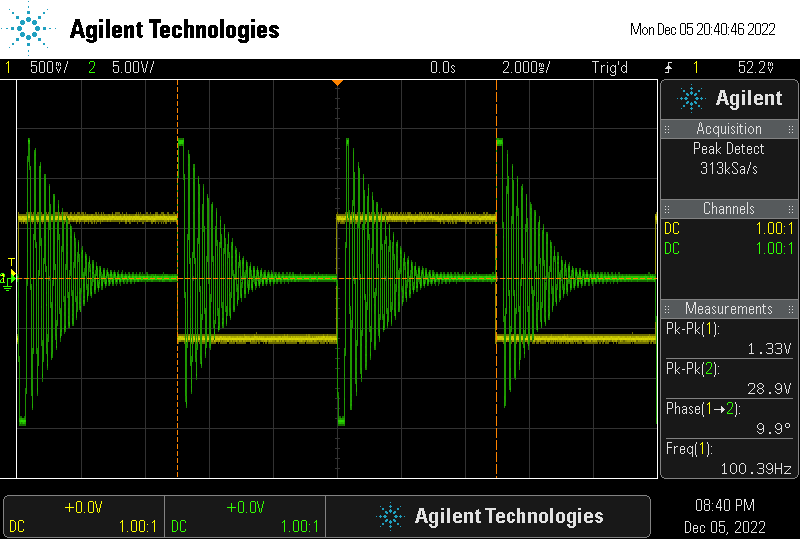
\includegraphics[width=\textwidth]{data/dif_rechteck.png}
        \subcaption{Das Eingangssignals ist eine Rechteckspannung, das Ausgangssignal eine gedämpfte Schwingung.}
    \end{subfigure}
    \hfill
    \begin{subfigure}{0.49\linewidth}%
        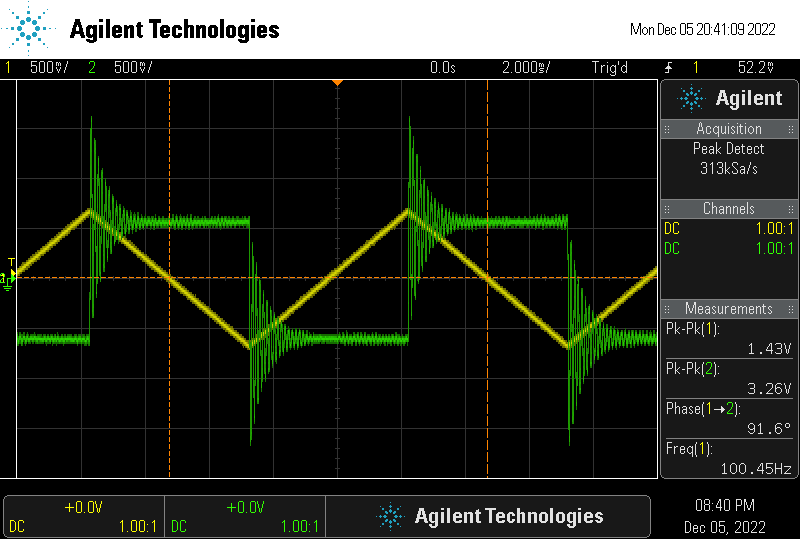
\includegraphics[width=\textwidth]{data/dif_dreieck.png}
        \subcaption{Das Eingangssignals ist eine Dreiecksspannung, das Ausgangssignal ist eine Rechteckspannung überlagert mit einer gedämpften Schwingung.}
    \end{subfigure}\\
    \begin{subfigure}{0.49\linewidth}%
        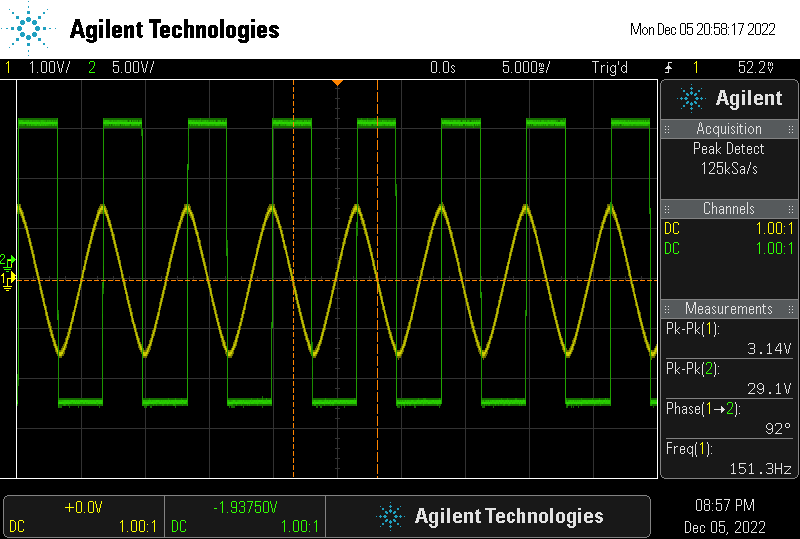
\includegraphics[width=\textwidth]{data/dif_sinus.png}
        \subcaption{Das Eingangssignal ist eine Sinusspannung, das Ausgangssignal ist ein Cosinussignal.}
    \end{subfigure}
    \caption{Die Bildschirmfotos des Oszilloskop bei verschiedenen Eingangssignals und Ausgangssignalen.
    Das gelbe Signal ist dabei immer das Eingangssignals des invertierenden-Differenzieres, das grüne Signal ist das Ausgangssignal der Schaltung.}
    \label{fig:dif_oszi}
\end{figure}